\documentclass[11pt,fleqn]{article}
\usepackage{../cs70,latexsym,epsf, amsmath,amsfonts,graphicx,url}
\lecture{10}
\def\title{Note \the\lecturenumber}
\begin{document}
\maketitle


\renewcommand{\F}{\mathbb{F}}
\renewcommand{\Z}{\mathbb{Z}}
\renewcommand{\Q}{\mathbb{Q}}
\renewcommand{\R}{\mathbb{R}}
\renewcommand{\N}{\mathbb{N}}
\newcommand{\C}{\mathbb{C}}


\section*{Infinity and Countability}

\noindent
\subsection*{Cardinality}

How can we determine whether two sets have the same {\it cardinality\/} (or
``size'')?
The answer to this question, reassuringly, lies in early grade school
memories: by demonstrating a {\it pairing\/} between elements of the two sets.
More formally, we need to demonstrate a {\it bijection\/}~$f$ between the two sets.
The bijection sets up a one-to-one correspondence, or pairing, between elements of
the two sets. We know how this works for finite sets.
In this lecture, we will see what it tells us about {\it infinite\/} sets.

Are there more natural numbers $\mathbb{N}$ than there are positive integers
$\mathbb{Z^+}$? It is tempting to answer yes, since every positive integer is
also a natural number, but the natural numbers have one extra element
$0 \notin \mathbb{Z^+}$. Upon more careful observation, though, we see that we can
generate a mapping between the natural numbers and the positive integers as follows:

\vbox{
\vspace{.1cm}
$\mathbb{N}$ \hspace{2.22cm} 0 \hspace{.3cm} 1 \hspace{.3cm} 2 \hspace{.3cm} 3 \hspace{.3cm} 4 \hspace{.3cm} 5 \hspace{.3cm} \ldots

\hspace{.5mm}$\downarrow$ \hspace{2.6cm} $\searrow$ \hspace{.1cm} $\searrow$ \hspace{.1cm} $\searrow$ \hspace{.1cm} $\searrow$ \hspace{.1cm} $\searrow$ \hspace{.1cm} $\searrow$

$\mathbb{Z^+}$ \hspace{2.75cm} 1 \hspace{.3cm} 2 \hspace{.3cm} 3 \hspace{.3cm} 4 \hspace{.3cm} 5 \hspace{.3cm} 6 \hspace{.3cm} \ldots
\vspace{.1cm}
}

Why is this mapping a bijection?  Clearly, the function
$f: \mathbb{N} \rightarrow \mathbb{Z^+}$ is onto because every positive integer
is hit.  And it is also one-to-one because no two natural numbers have the
same image.  (The image of $n$ is $f(n)=n+1$, so if $f(n)=f(m)$ then we must
have $n=m$.)
Since we have shown a bijection between $\mathbb{N}$ and $\mathbb{Z^{+}}$, this tells us
that there are as many natural numbers as there are positive integers!
Informally, we have proved that ``$\infty + 1 = \infty$."

What about the set of {\it even\/} natural numbers $2\mathbb{N} = \{0,2,4,6,...\}$?
In the previous example the difference was just one element. But in this example, there
seem to be twice as many natural numbers as there are even natural numbers. Surely,
the cardinality of $\mathbb{N}$ must be larger than that of $2\mathbb{N}$ since
$\mathbb{N}$ contains all of the odd natural numbers as well.
Though it might seem to be a more difficult task, let us attempt to find a bijection
between the two sets using the following mapping:

\vspace{.1cm}
$\mathbb{N}$ \hspace{2.22cm} 0 \hspace{.3cm} 1 \hspace{.3cm} 2 \hspace{.3cm} 3 \hspace{.3cm} 4 \hspace{.3cm} 5 \hspace{.3cm} \ldots

\hspace{.5mm}$\downarrow$ \hspace{2.26cm} $\downarrow$ \hspace{.3cm} $\downarrow$ \hspace{.3cm} $\downarrow$ \hspace{.3cm} $\downarrow$ \hspace{.3cm} $\downarrow$ \hspace{.3cm} $\downarrow$

$2\mathbb{N}$ \hspace{2.04cm} 0 \hspace{.3cm} 2 \hspace{.3cm} 4 \hspace{.3cm} 6 \hspace{.3cm} 8 \hspace{.2cm} 10 \hspace{.3cm} \ldots
\vspace{.1cm}


The mapping in this example is also a bijection. $f$ is clearly one-to-one, since
distinct natural numbers get mapped to distinct even natural numbers (because $f(n)=2n$).
$f$~is also onto, since every $n$ in the range is hit: its pre-image is
$\frac{n}{2}$.  Since we have found a bijection between these two sets, this tells us
that in fact $\mathbb{N}$ and $2\mathbb{N}$ have the same cardinality!

What about the set of all integers, $\mathbb{Z}$? At first glance, it may seem
obvious that the set of integers
is larger than the set of natural numbers, since it includes negative numbers.
However, as it turns out, it is possible
to find a bijection between the two sets, meaning that the two sets have the same
size! Consider the following mapping:

\vspace{.1cm}
0 $\rightarrow$ 0, ~ 1 $\rightarrow$  $-1$, ~ 2 $\rightarrow$  1, ~ 3
$\rightarrow$  $-2$, ~ 4 $\rightarrow$  2, \; \ldots, ~ 124 $\rightarrow$ 62, \;
\ldots
\vspace{.1cm}

In other words, our function is defined as follows:
$$
f(x) = \left\{
\begin{array}{cc}
\frac{x}{2}&\:\mbox{ if } x$ is even$\\
\frac{-(x+1)}{2} &\mbox{ if } x$ is odd$
\end{array}\right.
$$

We will prove that this function $f: \mathbb{N} \rightarrow \mathbb{Z}$ is a
bijection, by first showing that it is one-to-one and then showing that it is onto.

\noindent \textbf{Proof (one-to-one):} Suppose $f(x) = f(y)$. Then they both
must have the same sign. Therefore either $f(x) = \frac{x}{2}$ and $f(y) =
\frac{y}{2}$, or $f(x) = \frac{-(x+1)}{2}$ and $f(y) = \frac{-(y+1)}{2}$.
In the first case, $f(x) = f(y) \Rightarrow \frac{x}{2} = \frac{y}{2} \Rightarrow x =y$.
Hence $x=y$.  In the second case, $f(x) = f(y) \Rightarrow \frac{-(x+1)}{2} =
\frac{-(y+1)}{2} \Rightarrow x = y$.  So in both cases $f(x)=f(y) \Rightarrow x=y$,
so $f$ is injective.

\noindent \textbf{Proof (onto):} If $y\in\mathbb{Z}$ is non-negative, then $f(2y) = y$. Therefore,
$y$ has a pre-image. If $y$ is negative,
then $f(-(2y+1)) = y$. Therefore, $y$ has a pre-image. Thus every $y\in\mathbb{Z}$ has
a preimage, so $f$ is onto.

Since $f$ is a bijection, this tells us that $\mathbb{N}$ and $\mathbb{Z}$
have the same size.

Now for an important definition.  We say that a set~$S$ is {\bf countable} if there
is a bijection between~$S$ and $\mathbb{N}$ or some subset of~$\mathbb{N}$.  Thus
any finite set~$S$ is countable (since there is a bijection between $S$ and
the subset $\{0,1,2,\ldots,m-1\}$, where $m=|S|$ is the size of~$S$).  And we
have already seen three examples of countable infinite sets: $\mathbb{Z^+}$ and
$2\mathbb{N}$ are obviously countable since they are themselves subsets of~$\mathbb{N}$;
and $\mathbb{Z}$ is countable because we have just seen a bijection between it
and~$\mathbb{N}$.

What about the set of all rational numbers? Recall that $\mathbb{Q} =
\{\frac{x}{y}$ $|$ $x,y \in \mathbb{Z}$, $y \not= 0$\}.
Surely there are more rational numbers than natural numbers?  After all, there
are infinitely many rational numbers between any two natural numbers.
Surprisingly, the two sets have the same cardinality! To see this, let us introduce
a slightly different way of comparing the cardinality of two sets.

If there is a one-to-one function $f:A \rightarrow B$, then the
cardinality of $A$ is less than or equal to that of $B$.
Now to show that the cardinality of $A$ and $B$ are the same
we can show that $|A| \leq |B|$ and $|B| \leq |A|$. This
corresponds to showing that there is a one-to-one function
$f: A \rightarrow B$ and a one-to-one function $g: B \rightarrow A$.
The existence of these two one-to-one functions implies that there
is a bijection $h: A \rightarrow B$, thus showing that $A$ and
$B$ have the same cardinality. The proof of this fact, which is
called the Cantor-Bernstein theorem, is actually quite hard, and
we will skip it here.

Back to comparing the natural numbers and the rationals. First it is
obvious that $|\mathbb{N}|\le |\mathbb{Q}|$ because $\mathbb{N}\subseteq\mathbb{Q}$.
So our goal now is to prove that also $|\mathbb{Q}|\le|\mathbb{N}|$.  To do this,
we must exhibit an injection  $f:\mathbb{Q}\to\mathbb{N}$. The following picture
of a spiral conveys the idea of this injection:

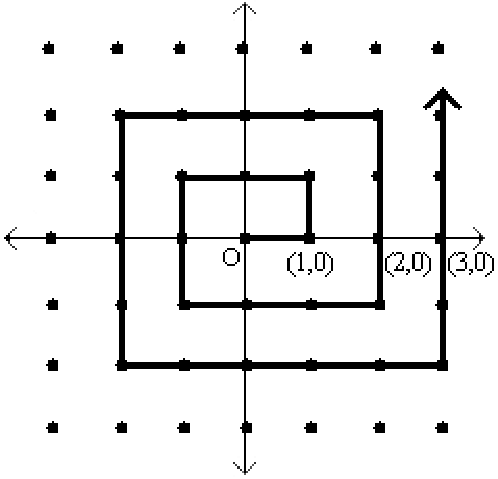
\includegraphics[scale = 0.7]{spiral}

Each rational number $\frac{a}{b}$ (written in its lowest terms, so that
$\gcd(a,b)=1$) is represented by the point $(a,b)$ in the infinite two-dimensional
grid shown (which corresponds to $\Z\times\Z$, the set of all pairs of integers).
Note that not all points on the grid are valid representations of rationals: e.g.,
all points on the $x$-axis have $b=0$ so none are valid (except for $(0,0)$, which
we take to represent the rational number~0); and points such as $(2,8)$ and $(-1,-4)$
are not valid either as the rational number $\frac{1}{4}$ is represented by $(1,4)$.
But $\Z\times \Z$ certainly contains all rationals under this representation, so if we
come up with an injection from $\Z\times \Z$ to~$\N$ then this will also be an
injection from~$\Q$ to~$\N$ (why?).

The idea is to map each pair $(a,b)$ to its position along the spiral, starting at
the origin.  (Thus, e.g.,$(0,0)\rightarrow 0$, $(1,0)\rightarrow 1$, $(1,1)\rightarrow 2$,
$(0,1)\rightarrow 3$, and so on.)  This mapping certainly maps every rational
number to a natural number, because every rational appears somewhere (exactly once)
in the grid, and the spiral hits every point in the grid.  Why is this mapping an injection?
Well, we just have to check that no two rational numbers map to the same natural
number.  But that is true because no two pairs lie at the same position on the spiral.
(Note that the mapping is {\it not\/} onto because some positions along the spiral
do not correspond to valid representations of rationals; but that is fine.)

This tells us that $|\mathbb{Q}| \leq |\mathbb{N}|$. Since
also $|\mathbb{N}| \leq |\mathbb{Q}|$, as we observed earlier, by the Cantor-Bernstein
Theorem $\mathbb{N}$ and $\mathbb{Q}$ have the same cardinality.

Our next example concerns the set of all binary strings (of any finite length),
denoted $\{0,1\}^*$.  Despite the fact that this set contains strings of unbounded length,
it turns out to have the same cardinality as~$\N$.  To see this, we set up a direct
bijection $f:\{0,1\}^*\to\N$ as follows.  Note that it suffices to {\it enumerate\/} the elements
of $\{0,1\}^*$ in such a way that each string appears exactly once in the list.  We then
get our bijection by setting $f(n)$ to be the $n$th string in the list.  How do we enumerate
the strings in $\{0,1\}^*$?  Well, it's natural to list them in increasing order of length, and
then (say) in {\it lexicographic\/} order (or, equivalently, numerically increasing order when
viewed as binary numbers) within the strings of each length.  This means that
the list would look like $$
   \varepsilon,0,1,00,01,10,11,000,001,010,011,100,101,110,111,1000,\ldots, $$
where $\varepsilon$ denotes the empty string (the only string of length~0).
It should be clear that this list contains each binary string once and only once, so we
get a bijection with~$\N$ as desired.

Our final countable example is the set of all polynomials with natural number
coefficients, which we denote $\N(x)$.  To see that this set is countable,
we will make use of (a variant of) the previous example.  Note first that, by essentially
the same argument as for $\{0,1\}^*$, we can see that the set of all {\it ternary\/}
strings $\{0,1,2\}^*$ (that is, strings over the alphabet $\{0,1,2\}$) is countable.
To see that $\N(x)$ is countable, it therefore suffices  to exhibit an injection
$f:\N(x)\to\{0,1,2\}^*$, which in turn will give an injection from $\N(x)$ to $\N$.
(It is obvious that there exists an injection from $\N$ to $\N(x)$,
since each natural number~$n$ is itself trivially a polynomial, namely the constant
polynomial $n$ itself.)

How do we define~$f$?  Let's first consider an example, namely the polynomial
$p(x) = 5x^5 + 2x^4 + 7x^3 + 4x + 6$.
We can list the coefficients of $p(x)$ as follows: $(5,2,7,0,4,6)$.
We can then write these coefficients as binary strings: $(101_2,10_2,111_2,0_2,100_2,110_2)$.
Now, we can construct a ternary string where a ``2" is inserted as a separator
between each binary coefficient (ignoring coefficients that are 0).
Thus we map $p(x)$ to a ternary string as illustrated below:

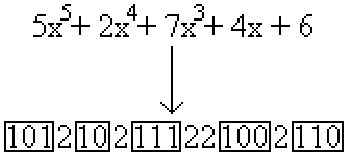
\includegraphics[bb = -90 0 0 80, scale = 0.7]{polynat}

It is easy to check that this is an injection, since the original polynomial can be uniquely
recovered from this ternary string by simply reading off the coefficients between each
successive pair of 2's.
(Notice that this mapping $f:\N(x)\to\{0,1,2\}^*$ is not onto (and
hence not a bijection) since many ternary strings will not be the image of any polynomials;
this will be the case, for example, for any ternary strings that contain binary subsequences
with leading zeros.)

Hence we have an injection from $\N(x)$ to~$\N$, so $\N(x)$ is countable.

\subsection*{Cantor's Diagonalization}

So we have established that $\mathbb{N}$, $\mathbb{Z}$, $\mathbb{Q}$
all have the same cardinality. What about the real numbers,
the set of all points on the real line? Surely they are countable too?
After all, the rational numbers, like the real numbers, are dense (i.e.,
between any two rational numbers there is a rational number):

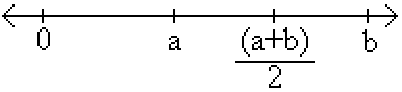
\includegraphics[bb = -100 0 0 50, scale = 0.7]{rationals}

In fact, between any two {\it real\/} numbers there is always a rational number.
It is really surprising, then, that there are more real numbers than
rationals. That is, there is no bijection between the rationals (or the
natural numbers) and the reals.
In fact, we will show something even stronger: even the real numbers
in the interval $[0,1]$ are uncountable!

Recall that a real number can be written out in an infinite decimal
expansion. A real number in the interval $[0,1]$ can be written
as $0.d_1 d_2 d_3$... Note that this representation is not unique; for example,
$1 = 0.999$...\footnote{To see this, write $x = .999 \ldots$.  Then
$10x = 9.999 \ldots$, so $9x = 9$, and thus $x=1$.}; for definiteness we
shall assume that every real number is represented as a recurring decimal
where possible (i.e., we choose the representation $.999\ldots$ rather
than $1$).

\textbf{Cantor's Diagonalization Proof:} Suppose towards a contradiction that there
is a bijection $f: \mathbb{N} \rightarrow \mathbb{R}[0,1]$.
Then, we can enumerate the infinite list as follows:

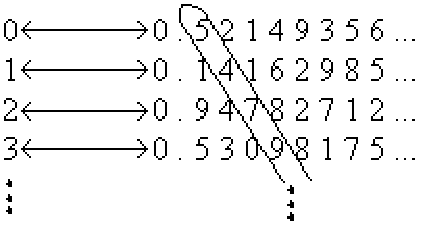
\includegraphics[bb = -40 0 0 115, scale = 0.7]{cantor}

\noindent The number circled in the diagonal is some real number
$D=0.5479\ldots$, since it is an infinite decimal expansion. Now
consider the real number $s$ obtained by modifying every digit of $r$,
say by replacing each digit $d$ with $d + 2 \bmod 10$; thus in our
example above, $s=0.7691\ldots$.  We claim that $s$ does not occur in
our infinite list of real numbers. Suppose for contradiction that it
did as the $n^{th}$ number in the list. But the $n$th number's
$n^{th}$ digit is the same as the $n^{th}$ digit of $r$ and thus is
different from the $n^{th}$ digit of $s$: the $n^{th}$ digit of $s$ is
the $n^{th}$ digit of $r$ plus $2 \bmod 10$. So we have a real number
$s$ that is not in the range of $f$. But this contradicts the
assertion that $f$ is a bijection. Thus the real numbers are not
countable.

Let us remark that the reason that we modified each digit by
adding $2 \bmod 10$ as opposed to adding $1$ is that the
same real number can have two decimal expansions; for example
$0.999$... $= 1.000$.... But if two real numbers differ by
more than $1$ in any digit they cannot be equal.  Thus we are
completely safe in our assertion.

With Cantor's diagonalization method, we proved that $\mathbb{R}$ is uncountable.
What happens if we apply the same method to $\mathbb{Q}$, in a (futile) attempt to show
the rationals are uncountable? Well, suppose for a contradiction that our bijective
function $f: \mathbb{N} \rightarrow \mathbb{Q} [0,1]$ produces the following mapping:

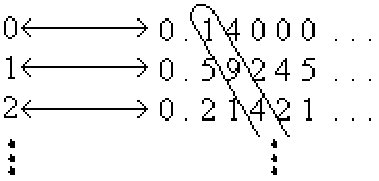
\includegraphics[bb = -40 0 0 90, scale = 0.7]{cantor3}

\noindent This time, let us consider the number $q$ obtained
by modifying every digit of the diagonal, say by replacing each digit $d$
with $d+2 \bmod 10$. Then in the above example $q$ = 0.316...,
and we want to try to show
that it does not occur in our infinite list of rational numbers. However, we
do not know if $q$ is rational (in fact, it is extremely unlikely for the
decimal expansion of $q$ to be periodic). This is why the method fails when applied
to the rationals. When dealing with the reals, the modified diagonal
number was guaranteed to be a real number.


\subsection*{The Cantor Set}
\textit{Please read on only if interested.}\\
The Cantor set is a remarkable set construction involving the real numbers in the interval
$[0,1]$. The set is defined by repeatedly removing the middle thirds of line segments infinitely many times,
starting with the original interval. For example, the first iteration would involve the removal of the interval $(\frac{1}{3},\frac{2}{3})$,
leaving $[0,\frac{1}{3}] \cup [\frac{2}{3},1]$. The first three iterations are illustrated below:

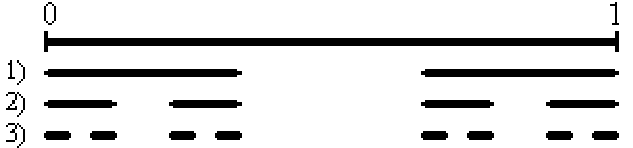
\includegraphics[bb = -40 0 0 75, scale = 0.7]{cantorset}

The Cantor set contains all points that have {\it not\/} been removed: $C = \{x : x$ not thrown out$\}$.
How much of the original unit interval is left after this process is repeated infinitely? Well, we start
with 1, and after the first iteration we remove $\frac{1}{3}$ of the interval, leaving us with $\frac{2}{3}$.
For the second iteration, we keep $\frac{2}{3}\times\frac{2}{3}$ of the original interval. As we repeat the
iterations infinitely, we are left with:

\vspace{.1cm}
$1 \longrightarrow \frac{2}{3} \longrightarrow \frac{2}{3} \times \frac{2}{3} \longrightarrow \frac{2}{3} \times \frac{2}{3} \times \frac{2}{3} \longrightarrow \cdots \longrightarrow \mathop {\lim }\limits_{n \to \infty } (\frac{2}{3})^n = 0$

According to the calculations, we have removed everything from the original interval!  Does this
mean that the Cantor set is empty?  No, it doesn't.  
What it means is that the {\it measure\/} of
the Cantor set is zero; the Cantor set consists of isolated points and does not contain any 
non-trivial intervals.  In fact, not only is the Cantor set non-empty, it is 
uncountable!\footnote{It's actually easy to see that $C$ contains at least countably many 
points, namely the endpoints of the intervals in the construction---i.e., numbers such as 
$\frac{1}{3}$, $\frac{2}{3}$, $\frac{1}{9}$, $\frac{1}{27}$ etc.  It's less obvious that $C$ also
contains various other points, such as $\frac{1}{4}$ and $\frac{3}{10}$.  (Why?)}

To see why, let us first make a few observations about ternary strings. In ternary
notation, all strings consist of digits (called ``trits") from the set $\{0,1,2\}$. All real numbers
in the interval $[0,1]$ can be written in ternary notation. (E.g., $\frac{1}{3}$ can be written as 
$0.1$, or equivalently as $0.0222\ldots$, and $\frac{2}{3}$ can be written as $0.2$ or
as $0.1222\ldots$.)  Thus, in the first iteration, the middle third removed contains
all ternary numbers of the form $0.1$xxxxx. The ternary numbers left after the first removal 
can all be expressed either in the form 0.0xxxxx... or 0.2xxxxx...
(We have to be a little careful here with the endpoints of the intervals; but we can
handle them by writing $\frac{1}{3}$ as $0.02222\ldots$ and $\frac{2}{3}$ as $0.2$.) 
The second iteration removes ternary numbers of the form 0.01xxxxx and 0.21xxxxx
(i.e., any number with 1 in the second position).
The third iteration removes 1's in the third position, and so on.  
Therefore, what remains is all ternary numbers with only 0's and 2's.  Thus we have
shown that $$
   C = \{x\in[0,1]:\hbox{\rm $x$ has a ternary representation consisting only of 0's and 2's}\}. $$
Finally, using this characterization, we can set up an {\it onto\/} map~$f$ from~$C$ to 
$[0,1]$.  Since we already know that $[0,1]$ is uncountable, this implies that $C$ is
uncountable also.  The map~$f$ is defined as follows: for $x\in C$, $f(x)$ is defined
as the binary decimal obtained by dividing each digit of the ternary representation of~$x$
by~2.  Thus, for example, if $x = 0.0220$ (in ternary), then $f(x)$ 
is the binary decimal $0.0110$).  But the set of all binary decimals 0.xxxxx$\ldots$
is in 1-1 correspondence with the real interval $[0,1]$, and the map $f$ is onto 
because every binary decimal is the image of some ternary string under~$f$ 
(obtained by doubling every binary digit).\footnote{Note that $f$ is {\it not\/}
injective; for example, the ternary strings $0.20222\ldots$ and $0.22$
map to binary strings $0.10111\ldots$ and $0.11$ respectively, which
denote the same real number.  Thus $f$ is not a bijection.  However, the current
proof shows that the cardinality of~$C$ is at least that of $[0,1]$, while it is obvious
that the cardinality of~$C$ is at most that of $[0,1]$ since $C\subset [0,1]$.  Hence
$C$ has the same cardinality as $[0,1]$ (and as $\R$).}    
This completes the proof that $C$ is uncountable.

\subsection*{Power Sets and Higher Orders of Infinity (Optional) }
\textit{Please read on only if interested.}\\
Let $S$ be any set. Then the {\it power set\/} of~$S$, denoted by $\mathcal{P}(S)$, is
the set of all subsets of $S$. More formally, it is defined as: $\mathcal{P}(S) = \{T :
T \subseteq S\}$. For example, if $S = \{1,2,3\}$, then $\mathcal{P}(S) =
\{\{\},\{1\},\{2\},\{3\},\{1,2\},\allowbreak\{1,3\},\allowbreak\{2,3\},\{1,2,3\}\}$. 

What is the cardinality of $\mathcal{P}(S)$? If $|S|=k$ is finite, 
then $|\mathcal{P}(S)| = 2^k$.
To see this, let us think of each subset of $S$ corresponding to a $k$ bit string. In the 
example above the subset $\{1,3\}$ corresponds to the string $101$. 
A $1$ in the $i^{th}$ position indicates that the $i^{th}$ element 
of $S$ is in the subset and a $0$ indicates that it is not. 
Now the number of binary strings of length $k$ is $2^k$, since 
there are two choices for each bit position. 
Thus $|\mathcal{P}(S)| = 2^{k}$. So for finite sets $S$, the cardinality of 
the power set of $S$ is exponentially larger than the cardinality of $S$. What about 
infinite (countable) sets? We claim that
there is no bijection from $S$ to $\mathcal{P}(S)$, so $\mathcal{P}(S)$ is
not countable.  Thus for example the set of all subsets of natural numbers
is not countable, even though the set of natural numbers itself is countable.

\textbf{Theorem:} Let $S$ be countably infinite.  Then $|\mathcal{P}(S)| > |S|$.

\textbf{Proof:} Suppose towards a contradiction that there is a bijection $f: S
\rightarrow \mathcal{P}(S)$. Recall that we can represent a subset by a binary
string, with one bit for each element of $S$. (So, since $S$ is infinite, the string
will be infinitely long.  Contrast the case of $\{0,1\}^*$ discussed earlier, which
consists of all binary strings of {\it finite\/} length.)  Consider the following
diagonalization picture in which the function $f$ maps natural numbers $x$
to binary strings which correspond to subsets of $S$ (e.g., 2 $\rightarrow$ 10100... $=$ \{0,2\}):

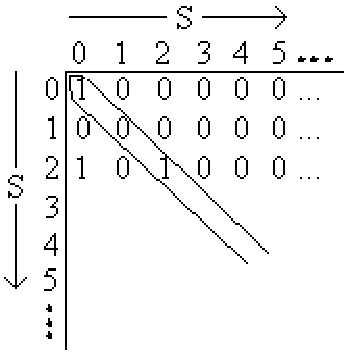
\includegraphics[bb = -40 0 0 170, scale = 0.7]{cantor2}

\noindent In this case, we have assigned the following mapping: 0 $\rightarrow$
\{0\}, 1 $\rightarrow$  \{\}, 2 $\rightarrow$ \{0,2\}, \ldots (i.e., the $n$th row describes
the $n^{th}$ subset as follows: if there is a 1 in the $k^{th}$ column, then $k$ is in
this subset, else it is not.)  Using a similar diagonalization argument to the earlier
one, flip each bit along the diagonal: 1 $\rightarrow$ 0, 0 $\rightarrow$ 1, and let 
$b$ denote the resulting binary string. First, we must show
that the new element is a subset of $S$. Clearly it is, since $b$ is an infinite
binary string which corresponds to a subset of $S$. Now suppose $b$ were the $n^{th}$
binary string. This cannot be the case though, since the $n^{th}$ bit of $b$ differs from
the  $n^{th}$ bit of the diagonal (the bits are flipped). So it's not on our list, but it should be, 
since we assumed that the list enumerated all possible subsets of $S$. Thus we 
have a contradiction, implying that  $\mathcal{P}(S)$ is uncountable.

Thus we have seen that the cardinality of $\mathcal{P}(\N)$ (the power set of the 
natural numbers) is strictly larger than the cardinality of $\N$ itself.  The cardinality
of~$\N$ is denoted $\aleph_0$ (pronounced ``aleph null"), while that of $\mathcal{P}(\N)$
is denoted $2^{\aleph_0}$.  It turns out that in fact $\mathcal{P}(\N)$ has the same
cardinality as~$\R$ (the real numbers), and indeed as the real numbers in $[0,1]$.
This cardinality is known as $\mathbf{c}$, the ``cardinality of the continuum."  So 
we know that $2^{\aleph_0}=\mathbf{c} > \aleph_0$.  Even larger infinite cardinalities 
(or ``orders of infinity"), denoted $\aleph_1,\aleph_2,\ldots$, can be defined using the 
machinery of set theory; these obey (to the uninitiated somewhat bizarre) rules of arithmetic.  
Several fundamental questions in modern mathematics concern these objects.
For example, the famous ``continuum hypothesis" asserts that $\mathbf{c}=\aleph_1$
(which is equivalent to saying that there are no sets with cardinality between that
of the natural numbers and that of the real numbers).

\end{document}
